

\renewcommand{\theequation}{\theenumi}
\begin{enumerate}[label=\arabic*.,ref=\thesubsection.\theenumi]
\numberwithin{equation}{enumi}

\item A pair of dice is thrown 4 times. If getting a doublet is considered a success, find the probability of two successes.\\
\item There are three coins. One is a two headed coin (having head on both faces), another is a biased coin that comes up heads 75$\%$ of the time and third is an unbiased coin. One of the three coins is chosen at random and tossed, it shows heads, what is the probability that it was the two headed coin ?\\

\item A fair coin and an unbiased die are tossed. Let A be the event ‘head appears on
the coin’ and B be the event ‘3 on the die’. Check whether A and B are independent events or not.\\\item An insurance company selected 2000 drivers at random (i.e., without
any preference of one driver over another) in a particular city to find a relationship between age and accidents. The data obtained are given in the Table \ref{table:prob_exam8}.
Find the probabilities of the following events for a driver chosen at random from the city:\\
(i) being 18-29 years of age \textit{and} having exactly 3 accidents in one year.\\
(ii) being 30-50 years of age \textit{and} having one or more accidents in a year.\\
(iii) having no accidents in one year.\\
\begin{table}[!ht]
\centering
\resizebox{\columnwidth}{!}{
\begin{tabular}{|c|c|c|c|c|c|}
\hline
\textbf{Age of drivers} &\multicolumn{5}{c|}{\textbf{Accidents in one year }}\\
\cline{2-6}
(in years) &\textbf{0} &\textbf{1} &\textbf{2} &\textbf{3} &\textbf{over 3}\\
\hline
18-29 &440 &160 &110 &61 &35\\
\hline
30-50 &505 &125 &60 &22 &18\\
\hline
Above 50 &360 &45 &35 &15 &9\\
\hline
\end{tabular}
}
\caption{}
\label{table:prob_exam8}
\end{table}

\solution
See Table \ref{table:2.1.8_sol}
 \begin{table}[!ht]
	\centering
	%%%%%%%%%%%%%%%%%%%%%%%%%%%%%%%%%%%%%%%%%%%%%%%%%%%%%%%%%%%%%%%%%%%%%%
%%                                                                  %%
%%  This is the header of a LaTeX2e file exported from Gnumeric.    %%
%%                                                                  %%
%%  This file can be compiled as it stands or included in another   %%
%%  LaTeX document. The table is based on the longtable package so  %%
%%  the longtable options (headers, footers...) can be set in the   %%
%%  preamble section below (see PRAMBLE).                           %%
%%                                                                  %%
%%  To include the file in another, the following two lines must be %%
%%  in the including file:                                          %%
%%        \def\inputGnumericTable{}                                 %%
%%  at the beginning of the file and:                               %%
%%        \input{name-of-this-file.tex}                             %%
%%  where the table is to be placed. Note also that the including   %%
%%  file must use the following packages for the table to be        %%
%%  rendered correctly:                                             %%
%%    \usepackage[latin1]{inputenc}                                 %%
%%    \usepackage{color}                                            %%
%%    \usepackage{array}                                            %%
%%    \usepackage{longtable}                                        %%
%%    \usepackage{calc}                                             %%
%%    \usepackage{multirow}                                         %%
%%    \usepackage{hhline}                                           %%
%%    \usepackage{ifthen}                                           %%
%%  optionally (for landscape tables embedded in another document): %%
%%    \usepackage{lscape}                                           %%
%%                                                                  %%
%%%%%%%%%%%%%%%%%%%%%%%%%%%%%%%%%%%%%%%%%%%%%%%%%%%%%%%%%%%%%%%%%%%%%%



%%  This section checks if we are begin input into another file or  %%
%%  the file will be compiled alone. First use a macro taken from   %%
%%  the TeXbook ex 7.7 (suggestion of Han-Wen Nienhuys).            %%
\def\ifundefined#1{\expandafter\ifx\csname#1\endcsname\relax}


%%  Check for the \def token for inputed files. If it is not        %%
%%  defined, the file will be processed as a standalone and the     %%
%%  preamble will be used.                                          %%
\ifundefined{inputGnumericTable}

%%  We must be able to close or not the document at the end.        %%
	\def\gnumericTableEnd{\end{document}}


%%%%%%%%%%%%%%%%%%%%%%%%%%%%%%%%%%%%%%%%%%%%%%%%%%%%%%%%%%%%%%%%%%%%%%
%%                                                                  %%
%%  This is the PREAMBLE. Change these values to get the right      %%
%%  paper size and other niceties.                                  %%
%%                                                                  %%
%%%%%%%%%%%%%%%%%%%%%%%%%%%%%%%%%%%%%%%%%%%%%%%%%%%%%%%%%%%%%%%%%%%%%%

	\documentclass[12pt%
			  %,landscape%
                    ]{report}
       \usepackage[latin1]{inputenc}
       \usepackage{fullpage}
       \usepackage{color}
       \usepackage{array}
       \usepackage{longtable}
       \usepackage{calc}
       \usepackage{multirow}
       \usepackage{hhline}
       \usepackage{ifthen}

	\begin{document}


%%  End of the preamble for the standalone. The next section is for %%
%%  documents which are included into other LaTeX2e files.          %%
\else

%%  We are not a stand alone document. For a regular table, we will %%
%%  have no preamble and only define the closing to mean nothing.   %%
    \def\gnumericTableEnd{}

%%  If we want landscape mode in an embedded document, comment out  %%
%%  the line above and uncomment the two below. The table will      %%
%%  begin on a new page and run in landscape mode.                  %%
%       \def\gnumericTableEnd{\end{landscape}}
%       \begin{landscape}


%%  End of the else clause for this file being \input.              %%
\fi

%%%%%%%%%%%%%%%%%%%%%%%%%%%%%%%%%%%%%%%%%%%%%%%%%%%%%%%%%%%%%%%%%%%%%%
%%                                                                  %%
%%  The rest is the gnumeric table, except for the closing          %%
%%  statement. Changes below will alter the table's appearance.     %%
%%                                                                  %%
%%%%%%%%%%%%%%%%%%%%%%%%%%%%%%%%%%%%%%%%%%%%%%%%%%%%%%%%%%%%%%%%%%%%%%

\providecommand{\gnumericmathit}[1]{#1} 
%%  Uncomment the next line if you would like your numbers to be in %%
%%  italics if they are italizised in the gnumeric table.           %%
%\renewcommand{\gnumericmathit}[1]{\mathit{#1}}
\providecommand{\gnumericPB}[1]%
{\let\gnumericTemp=\\#1\let\\=\gnumericTemp\hspace{0pt}}
 \ifundefined{gnumericTableWidthDefined}
        \newlength{\gnumericTableWidth}
        \newlength{\gnumericTableWidthComplete}
        \newlength{\gnumericMultiRowLength}
        \global\def\gnumericTableWidthDefined{}
 \fi
%% The following setting protects this code from babel shorthands.  %%
 \ifthenelse{\isundefined{\languageshorthands}}{}{\languageshorthands{english}}
%%  The default table format retains the relative column widths of  %%
%%  gnumeric. They can easily be changed to c, r or l. In that case %%
%%  you may want to comment out the next line and uncomment the one %%
%%  thereafter                                                      %%
\providecommand\gnumbox{\makebox[0pt]}
%%\providecommand\gnumbox[1][]{\makebox}

%% to adjust positions in multirow situations                       %%
\setlength{\bigstrutjot}{\jot}
\setlength{\extrarowheight}{\doublerulesep}

%%  The \setlongtables command keeps column widths the same across  %%
%%  pages. Simply comment out next line for varying column widths.  %%
\setlongtables

\setlength\gnumericTableWidth{%
	70pt+%
	70pt+%
	70pt+%
0pt}
\def\gumericNumCols{3}
\setlength\gnumericTableWidthComplete{\gnumericTableWidth+%
         \tabcolsep*\gumericNumCols*2+\arrayrulewidth*\gumericNumCols}
\ifthenelse{\lengthtest{\gnumericTableWidthComplete > \linewidth}}%
         {\def\gnumericScale{\ratio{\linewidth-%
                        \tabcolsep*\gumericNumCols*2-%
                        \arrayrulewidth*\gumericNumCols}%
{\gnumericTableWidth}}}%
{\def\gnumericScale{1}}

%%%%%%%%%%%%%%%%%%%%%%%%%%%%%%%%%%%%%%%%%%%%%%%%%%%%%%%%%%%%%%%%%%%%%%
%%                                                                  %%
%% The following are the widths of the various columns. We are      %%
%% defining them here because then they are easier to change.       %%
%% Depending on the cell formats we may use them more than once.    %%
%%                                                                  %%
%%%%%%%%%%%%%%%%%%%%%%%%%%%%%%%%%%%%%%%%%%%%%%%%%%%%%%%%%%%%%%%%%%%%%%

\ifthenelse{\isundefined{\gnumericColA}}{\newlength{\gnumericColA}}{}\settowidth{\gnumericColA}{\begin{tabular}{@{}p{70pt*\gnumericScale}@{}}x\end{tabular}}
\ifthenelse{\isundefined{\gnumericColB}}{\newlength{\gnumericColB}}{}\settowidth{\gnumericColB}{\begin{tabular}{@{}p{70pt*\gnumericScale}@{}}x\end{tabular}}
\ifthenelse{\isundefined{\gnumericColC}}{\newlength{\gnumericColC}}{}\settowidth{\gnumericColC}{\begin{tabular}{@{}p{70pt*\gnumericScale}@{}}x\end{tabular}}

\begin{tabular}[c]{%
	b{\gnumericColA}%
	b{\gnumericColB}%
	b{\gnumericColC}%
	}

%%%%%%%%%%%%%%%%%%%%%%%%%%%%%%%%%%%%%%%%%%%%%%%%%%%%%%%%%%%%%%%%%%%%%%
%%  The longtable options. (Caption, headers... see Goosens, p.124) %%
%	\caption{The Table Caption.}             \\	%
% \hline	% Across the top of the table.
%%  The rest of these options are table rows which are placed on    %%
%%  the first, last or every page. Use \multicolumn if you want.    %%

%%  Header for the first page.                                      %%
%	\multicolumn{3}{c}{The First Header} \\ \hline 
%	\multicolumn{1}{c}{colTag}	%Column 1
%	&\multicolumn{1}{c}{colTag}	%Column 2
%	&\multicolumn{1}{c}{colTag}	\\ \hline %Last column
%	\endfirsthead

%%  The running header definition.                                  %%
%	\hline
%	\multicolumn{3}{l}{\ldots\small\slshape continued} \\ \hline
%	\multicolumn{1}{c}{colTag}	%Column 1
%	&\multicolumn{1}{c}{colTag}	%Column 2
%	&\multicolumn{1}{c}{colTag}	\\ \hline %Last column
%	\endhead

%%  The running footer definition.                                  %%
%	\hline
%	\multicolumn{3}{r}{\small\slshape continued\ldots} \\
%	\endfoot

%%  The ending footer definition.                                   %%
%	\multicolumn{3}{c}{That's all folks} \\ \hline 
%	\endlastfoot
%%%%%%%%%%%%%%%%%%%%%%%%%%%%%%%%%%%%%%%%%%%%%%%%%%%%%%%%%%%%%%%%%%%%%%

\hhline{|-|-|-}
	 \multicolumn{1}{|p{\gnumericColA}|}%
	{\gnumericPB{\centering}class interval}
	&\multicolumn{1}{p{\gnumericColB}|}%
	{\gnumericPB{\centering}frequency}
	&\multicolumn{1}{p{\gnumericColC}|}%
	{\gnumericPB{\raggedright}cumulitive friquency}
\\
\hhline{|---|}
	 \multicolumn{1}{|p{\gnumericColA}|}%
	{\gnumericPB{\centering}0-100}
	&\multicolumn{1}{p{\gnumericColB}|}%
	{\gnumericPB{\centering}2}
	&\multicolumn{1}{p{\gnumericColC}|}%
	{\gnumericPB{\raggedleft}2}
\\
\hhline{|---|}
	 \multicolumn{1}{|p{\gnumericColA}|}%
	{\gnumericPB{\centering}100-200}
	&\multicolumn{1}{p{\gnumericColB}|}%
	{\gnumericPB{\centering}5}
	&\multicolumn{1}{p{\gnumericColC}|}%
	{\gnumericPB{\raggedleft}7}
\\
\hhline{|---|}
	 \multicolumn{1}{|p{\gnumericColA}|}%
	{\gnumericPB{\centering}200-300}
	&\multicolumn{1}{p{\gnumericColB}|}%
	{\gnumericPB{\centering}x}
	&\multicolumn{1}{p{\gnumericColC}|}%
	{\gnumericPB{\raggedright}7 + x}
\\
\hhline{|---|}
	 \multicolumn{1}{|p{\gnumericColA}|}%
	{\gnumericPB{\centering}300-400}
	&\multicolumn{1}{p{\gnumericColB}|}%
	{\gnumericPB{\centering}12}
	&\multicolumn{1}{p{\gnumericColC}|}%
	{\gnumericPB{\raggedright}19 + x}
\\
\hhline{|---|}
	 \multicolumn{1}{|p{\gnumericColA}|}%
	{\gnumericPB{\centering}400-500}
	&\multicolumn{1}{p{\gnumericColB}|}%
	{\gnumericPB{\centering}17}
	&\multicolumn{1}{p{\gnumericColC}|}%
	{\gnumericPB{\raggedright}36 +x}
\\
\hhline{|---|}
	 \multicolumn{1}{|p{\gnumericColA}|}%
	{\gnumericPB{\centering}500-600}
	&\multicolumn{1}{p{\gnumericColB}|}%
	{\gnumericPB{\centering}20}
	&\multicolumn{1}{p{\gnumericColC}|}%
	{\gnumericPB{\raggedright}56 + x}
\\
\hhline{|---|}
	 \multicolumn{1}{|p{\gnumericColA}|}%
	{\gnumericPB{\centering}600-700}
	&\multicolumn{1}{p{\gnumericColB}|}%
	{\gnumericPB{\centering}y}
	&\multicolumn{1}{p{\gnumericColC}|}%
	{\gnumericPB{\raggedright}56 +x+y}
\\
\hhline{|---|}
	 \multicolumn{1}{|p{\gnumericColA}|}%
	{\gnumericPB{\centering}700-800}
	&\multicolumn{1}{p{\gnumericColB}|}%
	{\gnumericPB{\centering}9}
	&\multicolumn{1}{p{\gnumericColC}|}%
	{\gnumericPB{\raggedright}65+x+y}
\\
\hhline{|---|}
	 \multicolumn{1}{|p{\gnumericColA}|}%
	{\gnumericPB{\centering}800-900}
	&\multicolumn{1}{p{\gnumericColB}|}%
	{\gnumericPB{\centering}7}
	&\multicolumn{1}{p{\gnumericColC}|}%
	{\gnumericPB{\raggedright}72+x+y}
\\
\hhline{|---|}
	 \multicolumn{1}{|p{\gnumericColA}|}%
	{\gnumericPB{\centering}900-1000}
	&\multicolumn{1}{p{\gnumericColB}|}%
	{\gnumericPB{\centering}4}
	&\multicolumn{1}{p{\gnumericColC}|}%
	{\gnumericPB{\raggedright}76+x+y}
\\
\hhline{|-|-|-|}
\end{tabular}

\ifthenelse{\isundefined{\languageshorthands}}{}{\languageshorthands{\languagename}}
\gnumericTableEnd

	\caption{}
\label{table:2.1.8_sol}
\end{table}

n = 100
\\
$implies$
\begin{align}
76 + x + y &= 100
\\
x+y = 24
\end{align}
class related to the Median 525 = 500-600
from anove we can say that 
\\
\begin{align}
l &= 500
\\
h = 100
\\
f= 20
\\
cf &= 36+x
\\
Median = l + \frac{\frac{n}{2} - cf}{f}\times h
\\
525 =  500 + \frac{50-36-x}{f}\times 100
\\
25 = 70-5x
\\
x = 9
\end{align}
from eq 3.8.1.2 and 3.8.1.10

\begin{align}
9 + y = 24
\\
y= 15
\end{align}
Related code is available in 
\begin{lstlisting}
solutions/1-10/codes/statexm/statexm8.py
\end{lstlisting}

\item A black and a red dice are rolled.\\
(a) Find the conditional probability of obtaining a sum greater than 9, given that the black die resulted in a 5.\\
(b) Find the conditional probability of obtaining the sum 8, given that the red die resulted in a number less than 4.\\
\solution
Let $Y_i \in \cbrak{1,2,3,4,5,6}$represent the outcome where $Y_1$ denotes black dice.

\begin{enumerate}
\item 
\begin{multline}
\pr{Y_1+Y_2 >9| Y_1 = 5} 
\\
= \frac{\pr{Y_1+Y_2 >9, Y_1 = 5}}{\pr{Y_1 = 5}}
\\
= \frac{\pr{Y_2 > 4, Y_1 = 5}}{\pr{Y_1 = 5}} 
\\
= \pr{Y_2 > 4} = \frac{1}{3}
\end{multline}
\item 
\begin{multline}
\pr{Y_1+Y_2 = 8| Y_2 < 4} 
\\
= \frac{\pr{Y_1 >4, Y_2 < 4}}{\pr{ Y_2 < 4}}
\\
=  \pr{Y_1 > 4} = \frac{1}{3}
\end{multline}
\end{enumerate}

\item In a hostel, 60$\%$ of the students read Hindi newspaper, 40$\%$ read English newspaper and 20$\%$ read both Hindi and English newspapers. A student is selected at random.\\
\\(a) Find the probability that she reads neither Hindi nor English newspapers.\\
\\(b) If she reads Hindi newspaper, find the probability that she reads English newspaper.\\
\\(c) If she reads English newspaper, find the probability that she reads Hindi newspaper.\\
\solution

General equation of conics is 
\begin{align}
    \vec{x}^T\vec{V}\vec{x}+ 2\vec{u}^T\vec{x}+f = 0
    \label{eq:solutions/1/16/eq:1}
\end{align}
Comparing with the equation given,
\begin{align}
\vec{V}=\myvec{\frac{1}{9} & 0 \\ 0 & \frac{1}{16}}\\
\vec{u}=\vec{0}\\
f=-1\\
\mydet{\vec{v}}=\mydet{\myvec{\frac{1}{9} & 0 \\ 0 & \frac{1}{16}}}>0
\end{align}
$\because \abs{\vec{V}}>0$, the given equation is of ellipse.\\
a)The tangents are parallel to the x-axis, hence, their direction and normal vectors, $\vec{m_1}$ and $\vec{n_1}$ are respectively,
\begin{align}
\vec{m_1}=\myvec{1\\0}\\
\vec{n_1}=\myvec{0\\1}
\end{align}
For an ellipse, given the normal vector $\vec{n}$, the tangent points of contact to the ellipse are given by
\begin{align}
    \vec{q}=\vec{V}^{-1}(\kappa \vec{n}-\vec{u})
    \label{eq:solutions/1/16/eq:2}
    =\vec{V}^{-1}\kappa \vec{n}
\end{align}
where
\begin{align}
    \kappa=\pm \sqrt{\frac{\vec{u^T}\vec{V}^{-1}\vec{u}-f}{\vec{n^T}\vec{V}^{-1}\vec{n}}}
    \label{eq:solutions/1/16/eq:2.0.9}\\
   =\pm \sqrt{\frac{-f}{\vec{n^T}\vec{V}^{-1}\vec{n}}}\\
    \vec{V}^{-1}=\myvec{9 & 0 \\ 0 & 16}\\
    \kappa_1=\pm \sqrt{\frac{-(-1)}{\myvec{0 & 1}\myvec{9 & 0 \\ 0 & 16} \myvec{0\\1}}}\\
 \implies \kappa_1=\pm \sqrt{\frac{1}{16}}\\
    \implies \kappa_1=\pm \frac{1}{4}      
\end{align}
From \eqref{eq:solutions/1/16/eq:2} , the point of contact $\vec{q_i}$ are,
\begin{align}
    \vec{q_1}=\myvec{9 & 0 \\ 0 & 16}\frac{1}{4}\myvec{0\\1}\\
    =\myvec{9 & 0 \\ 0 & 16}\myvec{0\\\frac{1}{4}}\\
    =\myvec{0\\4}\\
    \vec{q_2}=\myvec{9 & 0 \\ 0 & 16}\left(-\frac{1}{4}\right)\ \myvec{0\\1}\\
    =\myvec{9 & 0 \\ 0 & 16}\myvec{0\\-\frac{1}{4}}\\
    =\myvec{0\\-4}
\end{align}
b) The tangents are parallel to the y-axis, hence, their direction and normal vectors, $\vec{m_2}$ and $\vec{n_2}$ are respectively,
\begin{align}
\vec{m_2}=\myvec{0\\1}\\
\vec{n_2}=\myvec{1\\0}
\end{align}
Using equation \eqref{eq:solutions/1/16/eq:2.0.9}, the values of $\kappa$ for this case are
\begin{align}
     \kappa_2=\pm \sqrt{\frac{-(-1)}{\myvec{1 & 0}\myvec{9 & 0 \\ 0 & 16} \myvec{1\\0}}}\\
 \implies \kappa_2=\pm \sqrt{\frac{1}{9}}\\
    \implies \kappa_2=\pm \frac{1}{3} 
\end{align}
and from \eqref{eq:solutions/1/16/eq:2} , the point of contact $\vec{q_i}$ are,
\begin{align}
\vec{q_3}=\myvec{9 & 0 \\ 0 & 16}\frac{1}{3}\myvec{1\\0}\\
    =\myvec{9 & 0 \\ 0 & 16}\myvec{\frac{1}{3}\\0}\\
    =\myvec{3\\0}\\
\vec{q_4}=\myvec{9 & 0 \\ 0 & 16}\left(-\frac{1}{3}\right)\ \myvec{1\\0}\\
    =\myvec{9 & 0 \\ 0 & 16}\myvec{-\frac{1}{3}\\0}\\
    =\myvec{-3\\0}
\end{align}
 \begin{figure}[h!]
	\centering
	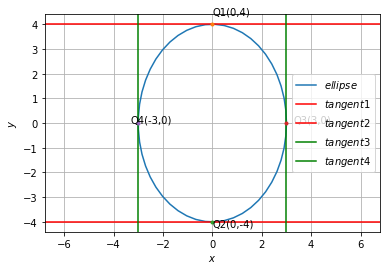
\includegraphics[width=\columnwidth]{./solutions/conics/1/16/ellipse.png}
	\caption{Figure depicting point of contact of tangents of ellipse parallel to x-axis and y-axis}
	\label{eq:solutions/1/16/fig1}
\end{figure}


Choose the correct answer: 
\item The probability of obtaining an even prime number on each die, when a pair of dice is rolled is
\begin{enumerate}
\item 0
\item $\frac{1}{3}$
\item $\frac{1}{12}$
\item $\frac{1}{36}$
\end{enumerate}
\solution

General equation of conics is 
\begin{align}
    \vec{x}^T\vec{V}\vec{x}+ 2\vec{u}^T\vec{x}+f = 0
    \label{eq:solutions/1/16/eq:1}
\end{align}
Comparing with the equation given,
\begin{align}
\vec{V}=\myvec{\frac{1}{9} & 0 \\ 0 & \frac{1}{16}}\\
\vec{u}=\vec{0}\\
f=-1\\
\mydet{\vec{v}}=\mydet{\myvec{\frac{1}{9} & 0 \\ 0 & \frac{1}{16}}}>0
\end{align}
$\because \abs{\vec{V}}>0$, the given equation is of ellipse.\\
a)The tangents are parallel to the x-axis, hence, their direction and normal vectors, $\vec{m_1}$ and $\vec{n_1}$ are respectively,
\begin{align}
\vec{m_1}=\myvec{1\\0}\\
\vec{n_1}=\myvec{0\\1}
\end{align}
For an ellipse, given the normal vector $\vec{n}$, the tangent points of contact to the ellipse are given by
\begin{align}
    \vec{q}=\vec{V}^{-1}(\kappa \vec{n}-\vec{u})
    \label{eq:solutions/1/16/eq:2}
    =\vec{V}^{-1}\kappa \vec{n}
\end{align}
where
\begin{align}
    \kappa=\pm \sqrt{\frac{\vec{u^T}\vec{V}^{-1}\vec{u}-f}{\vec{n^T}\vec{V}^{-1}\vec{n}}}
    \label{eq:solutions/1/16/eq:2.0.9}\\
   =\pm \sqrt{\frac{-f}{\vec{n^T}\vec{V}^{-1}\vec{n}}}\\
    \vec{V}^{-1}=\myvec{9 & 0 \\ 0 & 16}\\
    \kappa_1=\pm \sqrt{\frac{-(-1)}{\myvec{0 & 1}\myvec{9 & 0 \\ 0 & 16} \myvec{0\\1}}}\\
 \implies \kappa_1=\pm \sqrt{\frac{1}{16}}\\
    \implies \kappa_1=\pm \frac{1}{4}      
\end{align}
From \eqref{eq:solutions/1/16/eq:2} , the point of contact $\vec{q_i}$ are,
\begin{align}
    \vec{q_1}=\myvec{9 & 0 \\ 0 & 16}\frac{1}{4}\myvec{0\\1}\\
    =\myvec{9 & 0 \\ 0 & 16}\myvec{0\\\frac{1}{4}}\\
    =\myvec{0\\4}\\
    \vec{q_2}=\myvec{9 & 0 \\ 0 & 16}\left(-\frac{1}{4}\right)\ \myvec{0\\1}\\
    =\myvec{9 & 0 \\ 0 & 16}\myvec{0\\-\frac{1}{4}}\\
    =\myvec{0\\-4}
\end{align}
b) The tangents are parallel to the y-axis, hence, their direction and normal vectors, $\vec{m_2}$ and $\vec{n_2}$ are respectively,
\begin{align}
\vec{m_2}=\myvec{0\\1}\\
\vec{n_2}=\myvec{1\\0}
\end{align}
Using equation \eqref{eq:solutions/1/16/eq:2.0.9}, the values of $\kappa$ for this case are
\begin{align}
     \kappa_2=\pm \sqrt{\frac{-(-1)}{\myvec{1 & 0}\myvec{9 & 0 \\ 0 & 16} \myvec{1\\0}}}\\
 \implies \kappa_2=\pm \sqrt{\frac{1}{9}}\\
    \implies \kappa_2=\pm \frac{1}{3} 
\end{align}
and from \eqref{eq:solutions/1/16/eq:2} , the point of contact $\vec{q_i}$ are,
\begin{align}
\vec{q_3}=\myvec{9 & 0 \\ 0 & 16}\frac{1}{3}\myvec{1\\0}\\
    =\myvec{9 & 0 \\ 0 & 16}\myvec{\frac{1}{3}\\0}\\
    =\myvec{3\\0}\\
\vec{q_4}=\myvec{9 & 0 \\ 0 & 16}\left(-\frac{1}{3}\right)\ \myvec{1\\0}\\
    =\myvec{9 & 0 \\ 0 & 16}\myvec{-\frac{1}{3}\\0}\\
    =\myvec{-3\\0}
\end{align}
 \begin{figure}[h!]
	\centering
	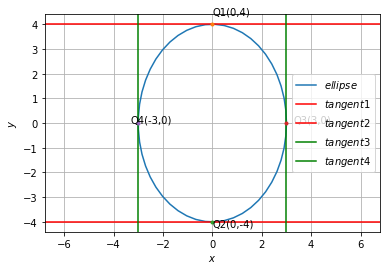
\includegraphics[width=\columnwidth]{./solutions/conics/1/16/ellipse.png}
	\caption{Figure depicting point of contact of tangents of ellipse parallel to x-axis and y-axis}
	\label{eq:solutions/1/16/fig1}
\end{figure}

\end{enumerate}

